\documentclass[fyma2,final]{prosper}
\usepackage[czech]{babel}
\usepackage[utf8]{inputenc}
\usepackage[T1]{fontenc}
\usepackage{graphicx}
\usepackage{pict2e}

\begin{document}
\title{Bezpečnostní protokoly}
\subtitle{Protokol Woo Lam $\Pi^f$}
\author{Pavel Frýz}
\email{xfryzp00@stud.fit.vutbr.cz}
\institution{Vysoké učení technické, Fakulta informačních technologií}
\displayVersion

\maketitle

\begin{slide}{Popis protokolu}
\begin{itemize}
 \item Vytvořen:
   \begin{itemize}
   \item Thomas Y.\,C.\,Woo a Simon S.\,Lam
   \item V roce 1994
   \end{itemize}
 \item Zajišťuje:
   \begin{itemize}
   \item Jednosměrnou autentizaci
   \item Autentizuje účastníka komunikace A(iniciátor spojení) vůči B.
   \end{itemize}
 \item Používá:
   \begin{itemize}
   \item Symetrickou kryptografie
   \item Důvěryhodný server
   \item Princip úplných informací
   \end{itemize}
\end{itemize}
\end{slide}

\begin{slide}{Reprezentace protokolu}
  \begin{tabular}{ll}
  \textbf{Textová reprezentace:}& \textbf{Grafická reprezentace:}\\

  \begin{minipage}[c]{0.49\textwidth}
    \begin{tabular}{ll}
    $A,B,S\colon$ & Subjekty\\
    $K_{AS},K_{BS}\colon$ & Sdílené klíče\\
    $N_B\colon$ & Nonce
    \end{tabular}
    \begin{enumerate}
    \item $A \rightarrow B\colon A$
    \item $B \rightarrow A\colon N_B$
    \item $A \rightarrow B\colon \{A,B,N_B\}_{K_{AS}}$
    \item $B \rightarrow S\colon \{A,B,N_B,$\\$\{A,B,N_B\}_{K_{AS}}\}_{K_{BS}}$
    \item $S \rightarrow B\colon \{A,B,N_B\}_{K_{BS}}$
    \end{enumerate}
    \begin{tabular}{|c|l|}\hline
    \multicolumn{2}{|c|}{\textbf{Počáteční znalosti}}\\\hline
    $A$ & $A, B, S, K_{AS}$\\\hline
    $B$ & $B, S, N_B, K_{BS}$\\\hline
    $S$ & $A, B, S, K_{AS}, K_{BS}$\\\hline
    \end{tabular}
  \end{minipage}
  &
  \begin{minipage}[c]{0.49\textwidth}
    \bigskip
    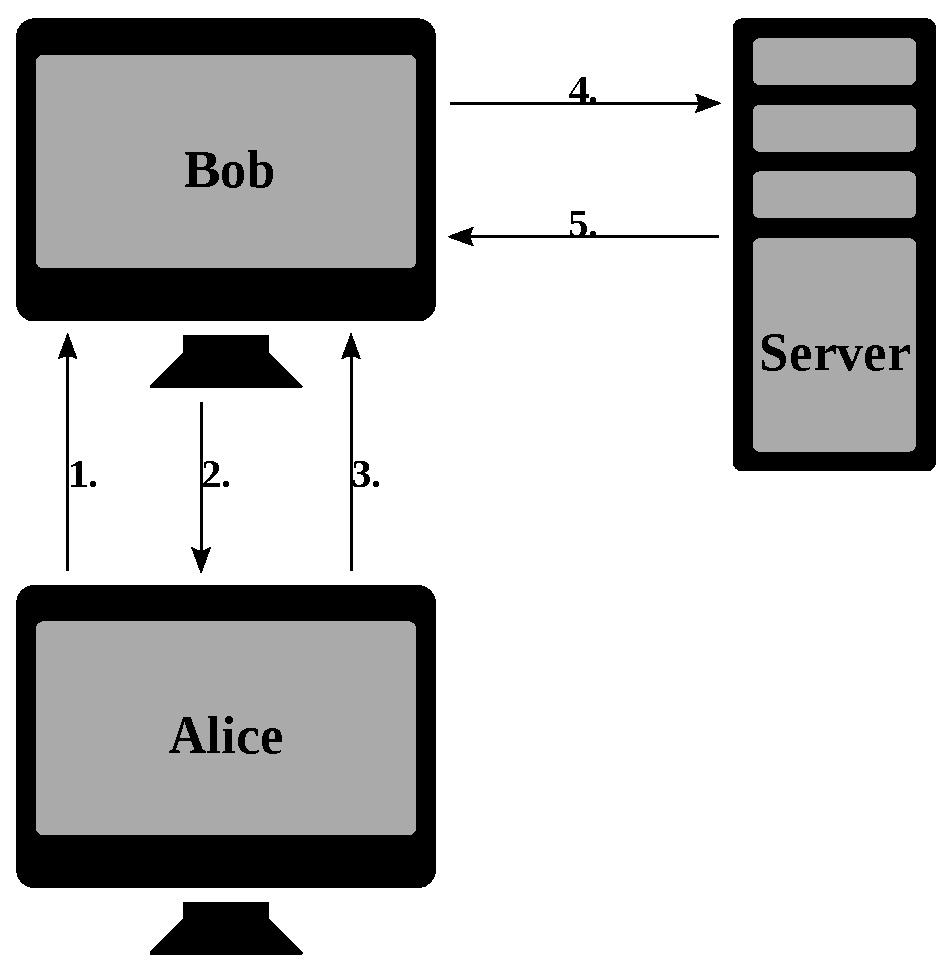
\includegraphics[width=0.85\textwidth]{reprezentace}
  \end{minipage}
  \end{tabular}
\end{slide}

\overlays{5}{
\begin{slide}{Průběh komunikace}
  \begin{figure}[p]
    \centering
    \setlength{\unitlength}{0.95mm}
   \begin{picture}(62,70)
      \thicklines
      \put(0,8){
        \put(0,4){\framebox(25,18){Alice}}
        \put(1,7){\framebox(23,13){}}
        \put(8,0){\line(1,1){2}}
        \put(10,2){\line(0,1){1}}
        \put(15,2){\line(0,1){1}}
        \put(10,3){\line(1,0){5}}
        \put(8,0){\line(1,0){9}}
        \put(17,0){\line(-1,1){2}}
      }
      \put(0,48){
        \put(0,4){\framebox(25,18){Bob}}
        \put(1,7){\framebox(23,13){}}
        \put(8,0){\line(1,1){2}}
        \put(10,2){\line(0,1){1}}
        \put(15,2){\line(0,1){1}}
        \put(10,3){\line(1,0){5}}
        \put(8,0){\line(1,0){9}}
        \put(17,0){\line(-1,1){2}}
      }
      \put(50,43){
        \put(0,0){\framebox(12,27){}}
        \put(1,1){\framebox(10,13){Server}}
        \put(1,15){\framebox(10,3){}}
        \put(1,19){\framebox(10,3){}}
        \put(1,23){\framebox(10,3){}}
      }
      \put(2,38){\makebox(4,5){1.}}
      \put(2,31){\vector(0,1){20}}
      \onlySlide*{1}{\put(0,0){\makebox(62,4)[l]{1: $A \rightarrow B\colon A$}}}
      \fromSlide{2}{
      \put(11,38){\makebox(4,5){2.}}
      \put(11,47){\vector(0,-1){16}}
      \onlySlide*{2}{\put(0,0){\makebox(62,4)[l]{2: $B \rightarrow A\colon N_B$}}}
      }
      \fromSlide{3}{
      \put(20,38){\makebox(4,5){3.}}
      \put(20,31){\vector(0,1){20}}
      \onlySlide*{3}{\put(0,0){\makebox(62,4)[l]{3: $A \rightarrow B\colon \{A,B,N_B\}_{K_{AS}}$}}}
      }
      \fromSlide{4}{
      \put(36,65){\makebox(4,4){4.}}
      \put(26,65){\vector(1,0){23}}
      \onlySlide*{4}{\put(0,0){\makebox(62,4)[l]{4: $B \rightarrow S\colon \{A,B,N_B,\{A,B,N_B\}_{K_{AS}}\}_{K_{BS}}$}}}
      }
      \fromSlide{5}{
      \put(36,58){\makebox(4,4){5.}}
      \put(49,58){\vector(-1,0){23}}
      \onlySlide*{5}{\put(0,0){\makebox(62,4)[l]{5: $S \rightarrow B\colon \{A,B,N_B\}_{K_{BS}}$}}}
      }
    \end{picture}
  \end{figure}
\end{slide}}

\begin{slide}{Použité zdroje}
\begin{itemize}
\item Repozitář bezpečnostních protokolů: \url{http://www.lsv.ens-cachan.fr/Software/spore/index.html}
\end{itemize}
\end{slide}


\end{document}
